\begin{pre}
	\thispagestyle{empty}
\begin{center}
  {\kaishu{材料来自于网上,如有侵权,请联系ocnzhao@163.com予以纠正,THX}}
\end{center}
\begin{center}
%		{\kaishu{人在春风和气中}}
\begin{figure}[htbp]
	\centering
	\includegraphics[width=0.5\textwidth]{Imagetreemath.png}
\end{figure}
\end{center}
\begin{center}
    本教案二维码下载地址: \qrcode[height=1in]{https://github.com/zggl/AITeachingPlanDraft2020/blob/master/AIMaster2020.pdf}
\end{center}
\begin{center}
%		{\kaishu{人在春风和气中}}
\begin{figure}[htbp]
	\centering
	\includegraphics[width=0.46\textwidth]{ImageAIwwl01.png}
    \includegraphics[width=0.45\textwidth]{ImageAIGQ.png}\\
    \includegraphics[width=0.45\textwidth]{ImageAILYR.png}
    \includegraphics[width=0.45\textwidth]{ImageAILDY.png}\\
\end{figure}
\begin{figure}[htbp]
    \includegraphics[width=0.45\textwidth]{ImageAISZZ.png}
    \includegraphics[width=0.45\textwidth]{ImageAIJQXX.png}
\end{figure}

史忠植——2013年凭借“拓展知识工程核心理论、创新分布智能理论基础、构建智能科学理论体系”成果, 荣获第三届吴文俊人工智能科学技术奖成就奖.

周志华——教育部“长江学者”特聘教授,国家杰出青年基金获得者;南京大学人工智能学院院长. 有一个旧称叫国立东南大学.
\end{center}

\href{https://www.sciencedaily.com/}{Science daily}

\paragraph{在线课程} 课程相关的电子材料存放平台和链接地址。

\href{https://gitee.com/zggl/AITeachingPlanDraft2020}{码云平台上的课程电子版和代码}

\href{https://github.com/zggl/AITeachingPlanDraft2020}{Github平台上的课程电子版和代码}

\href{https://ke.qq.com/webcourse/index.html?cid=1086628&term_id=101182654&lite=1&from=800021724#taid=5467185&vid=5285890799477964181}{1——人工智能基础-第一次 基础简介}

\href{https://ke.qq.com/webcourse/index.html?cid=1086628&term_id=101182654&lite=1&from=800021724#taid=8423279&vid=5285890799803709554}{2——人工智能基础-第二次-发展和应用}

\href{https://github.com/zggl/AITeachingPlanDraft2020/blob/master/3-\%E4\%BA\%BA\%E5\%B7\%A5\%E6\%99\%BA\%E8\%83\%BD\%E7\%AC\%AC\%E4\%BA\%8C\%E7\%AB\%A0\%E7\%AC\%AC\%E4\%B8\%80\%E6\%AC\%A1\%E5\%B9\%BB\%E7\%81\%AF\%20\%E4\%BA\%BA\%E5\%B7\%A5\%E6\%99\%BA\%E8\%83\%BD\%E7\%9A\%84\%E7\%9F\%A5\%E8\%AF\%86\%E8\%A1\%A8\%E7\%A4\%BA.pdf}{3——人工智能——知识表示}

\href{https://github.com/zggl/AITeachingPlanDraft2020/blob/master/4-\%E4\%BA\%BA\%E5\%B7\%A5\%E6\%99\%BA\%E8\%83\%BD\%E7\%AC\%AC\%E4\%B8\%89\%E7\%AB\%A0\%E7\%AC\%AC\%E4\%B8\%80\%E6\%AC\%A1\%20\%E4\%BA\%BA\%E5\%B7\%A5\%E6\%99\%BA\%E8\%83\%BD\%E7\%9A\%84\%E7\%9F\%A5\%E8\%AF\%86\%E6\%8E\%A8\%E7\%90\%86\%E6\%96\%B9\%E6\%B3\%95.pdf}{4——人工智能第三章——知识推理方法}
\href{https://edu.tipdm.org/notification?id=32302}{泰迪云课堂}

\href{http://speech.ee.ntu.edu.tw/~tlkagk/courses_ML20.html}{台大李宏毅老师的机器学习课程-2020}

\href{https://edu.tipdm.org/classroom/122/courses}{泰迪-深度学习原理及编程实现\_人邮版}


\href{https://deeplearn.org/}{Deep Learning Monitor}
%\vspace*{5\baselineskip}
%\centerline{\includegraphics[scale=0.6]{example/gzh.jpg}}
%\centerline{\fontsize{26pt}{26pt} 微信公众号}

自监督学习代码库:\href{https://github.com/open-mmlab/OpenSelfSup}{OpenSelfSup}

\href{http://alexlenail.me/NN-SVG/}{网络绘图工具}

\href{https://github.com/microsoft/tensorwatch}{Tensorwatch}, python的扩展包,作者随机产生的loss和accuracy,经过这个package的调用,将其动态显示成为图表

\href{https://www.engineeringonline.ncsu.edu/course/csc-520-artificial-intelligence-i/}{NCSU-CSC 520 Artificial Intelligence}

\href{https://cbovar.github.io/ConvNetDraw/}{ConvNetDraw(卷积神经网络),配置命令的CNN神经网络画图工具,开发者是香港的一位程序员。}

央视网,2020年07月12日 18:33, \href{https://tv.cctv.com/2020/07/12/VIDE97wmdEMDFTuh2C9XaSOL200712.shtml?spm=C53121759377.Pxm23GSMKB13.0.0}{《科幻地带》 20200712 科幻中的机器人(一)}

\href{https://scikit-learn.org/stable/about.html#citing-scikit-learn}{scikit-learn}

\href{https://createmomo.github.io/2018/01/23/Super-Machine-Learning-Revision-Notes/#tableofcontents}{Super Machine Learning Revision Notes }

\href{https://pytorch.org/assets/deep-learning/Deep-Learning-with-PyTorch.pdf}{Deep Learning With Pythons}
\begin{figure}[htbp]
    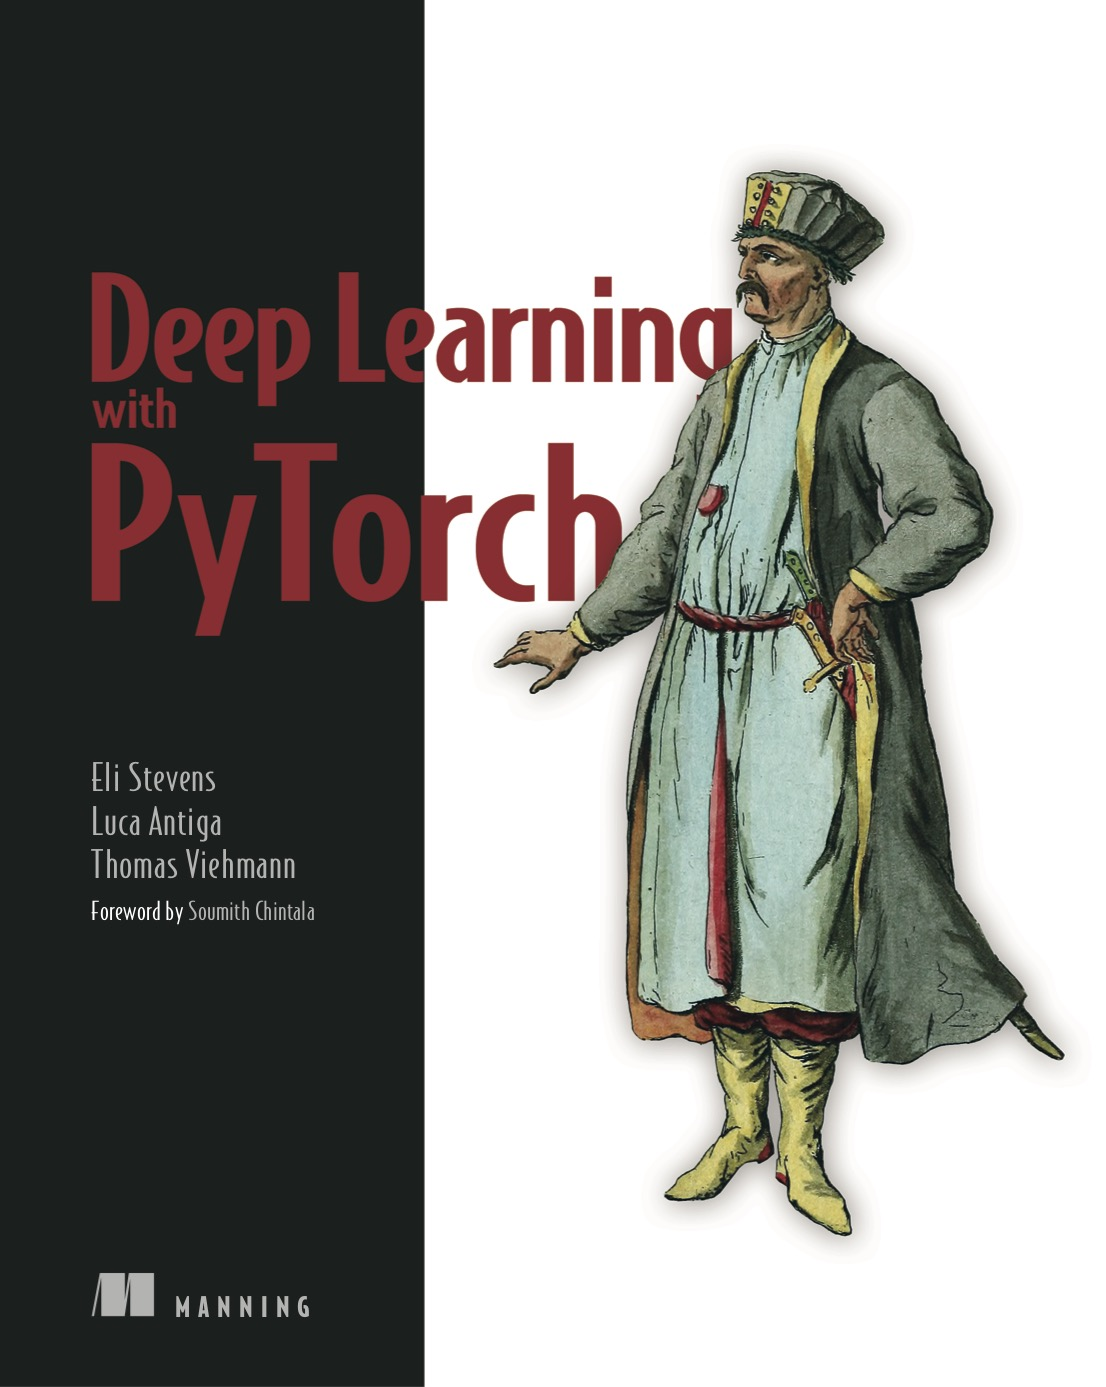
\includegraphics[width=0.45\textwidth]{deep-learning-thumbnail.png}
\end{figure}

48学时可以讲授到第七章

\subsection{NLP 2019相关顶会}
\href{https://github.com/zggl/NLP-Conferences-Code}{NLP 2019相关顶会}

\href{https://live.bilibili.com/21689802}{百度顶会论文复现营2020}
%%%%%--------------------------------------------------
\subsection{ICLR 2020}
International Conference on Learning Representation, 2020年4月26日在埃塞俄比亚的首都亚的斯亚贝巴开展。共收到了 2594 篇论文,接收了 687 篇,接收率为 26.5\%。

\href{https://openreview.net/forum?id=rJeB36NKvB}{How much position information do convolutional neural network encode?}
卷积神经网络是局部滤波器,它在有限的区域内通过调整卷积核参数来提取特征,这意味着卷积滤波器能输出对应某个特征的响应,但是以往的研究对于CNN是否同时也编码了位置信息没有给出证明。在这篇文章中,作者检验了这个假设,揭示了在CNN中编码的绝对位置信息的惊人程度。一组综合性的实验证明了这一假设的有效性,并揭示了在深层CNNs中,位置信息是从何而来,以及如何表达这些信息(\href{https://www.paperdigest.org/2019/12/iclr-2020-papers-with-code/}{ICLR2020开源代码的paper集合})。

工信安全: 2019年中国人工智能产业发展指数
\end{pre} 